\chapter{Phase III}

\section{Structur of software}
The figure \ref{fig:phase3} shows the implementation details behind the \emph{Opponent Model Strategy}. The \emph{Opponent Logger} tracks all the actions that are made by all players and associates them with the context at which these actions have been made. These actions are stored as list of \emph{Opponent Entry}-objects. 

At the showdown all the players that are still in the game have to show their cards. Now the \emph{Opponent Entry}-list of these players is went through. The player's cards are combined with the share cards and the hand strength is computed. The hand strength is committed to the \emph{Opponent Model} together with the current context and the player's action.

\begin{figure}[h]
  \centering
  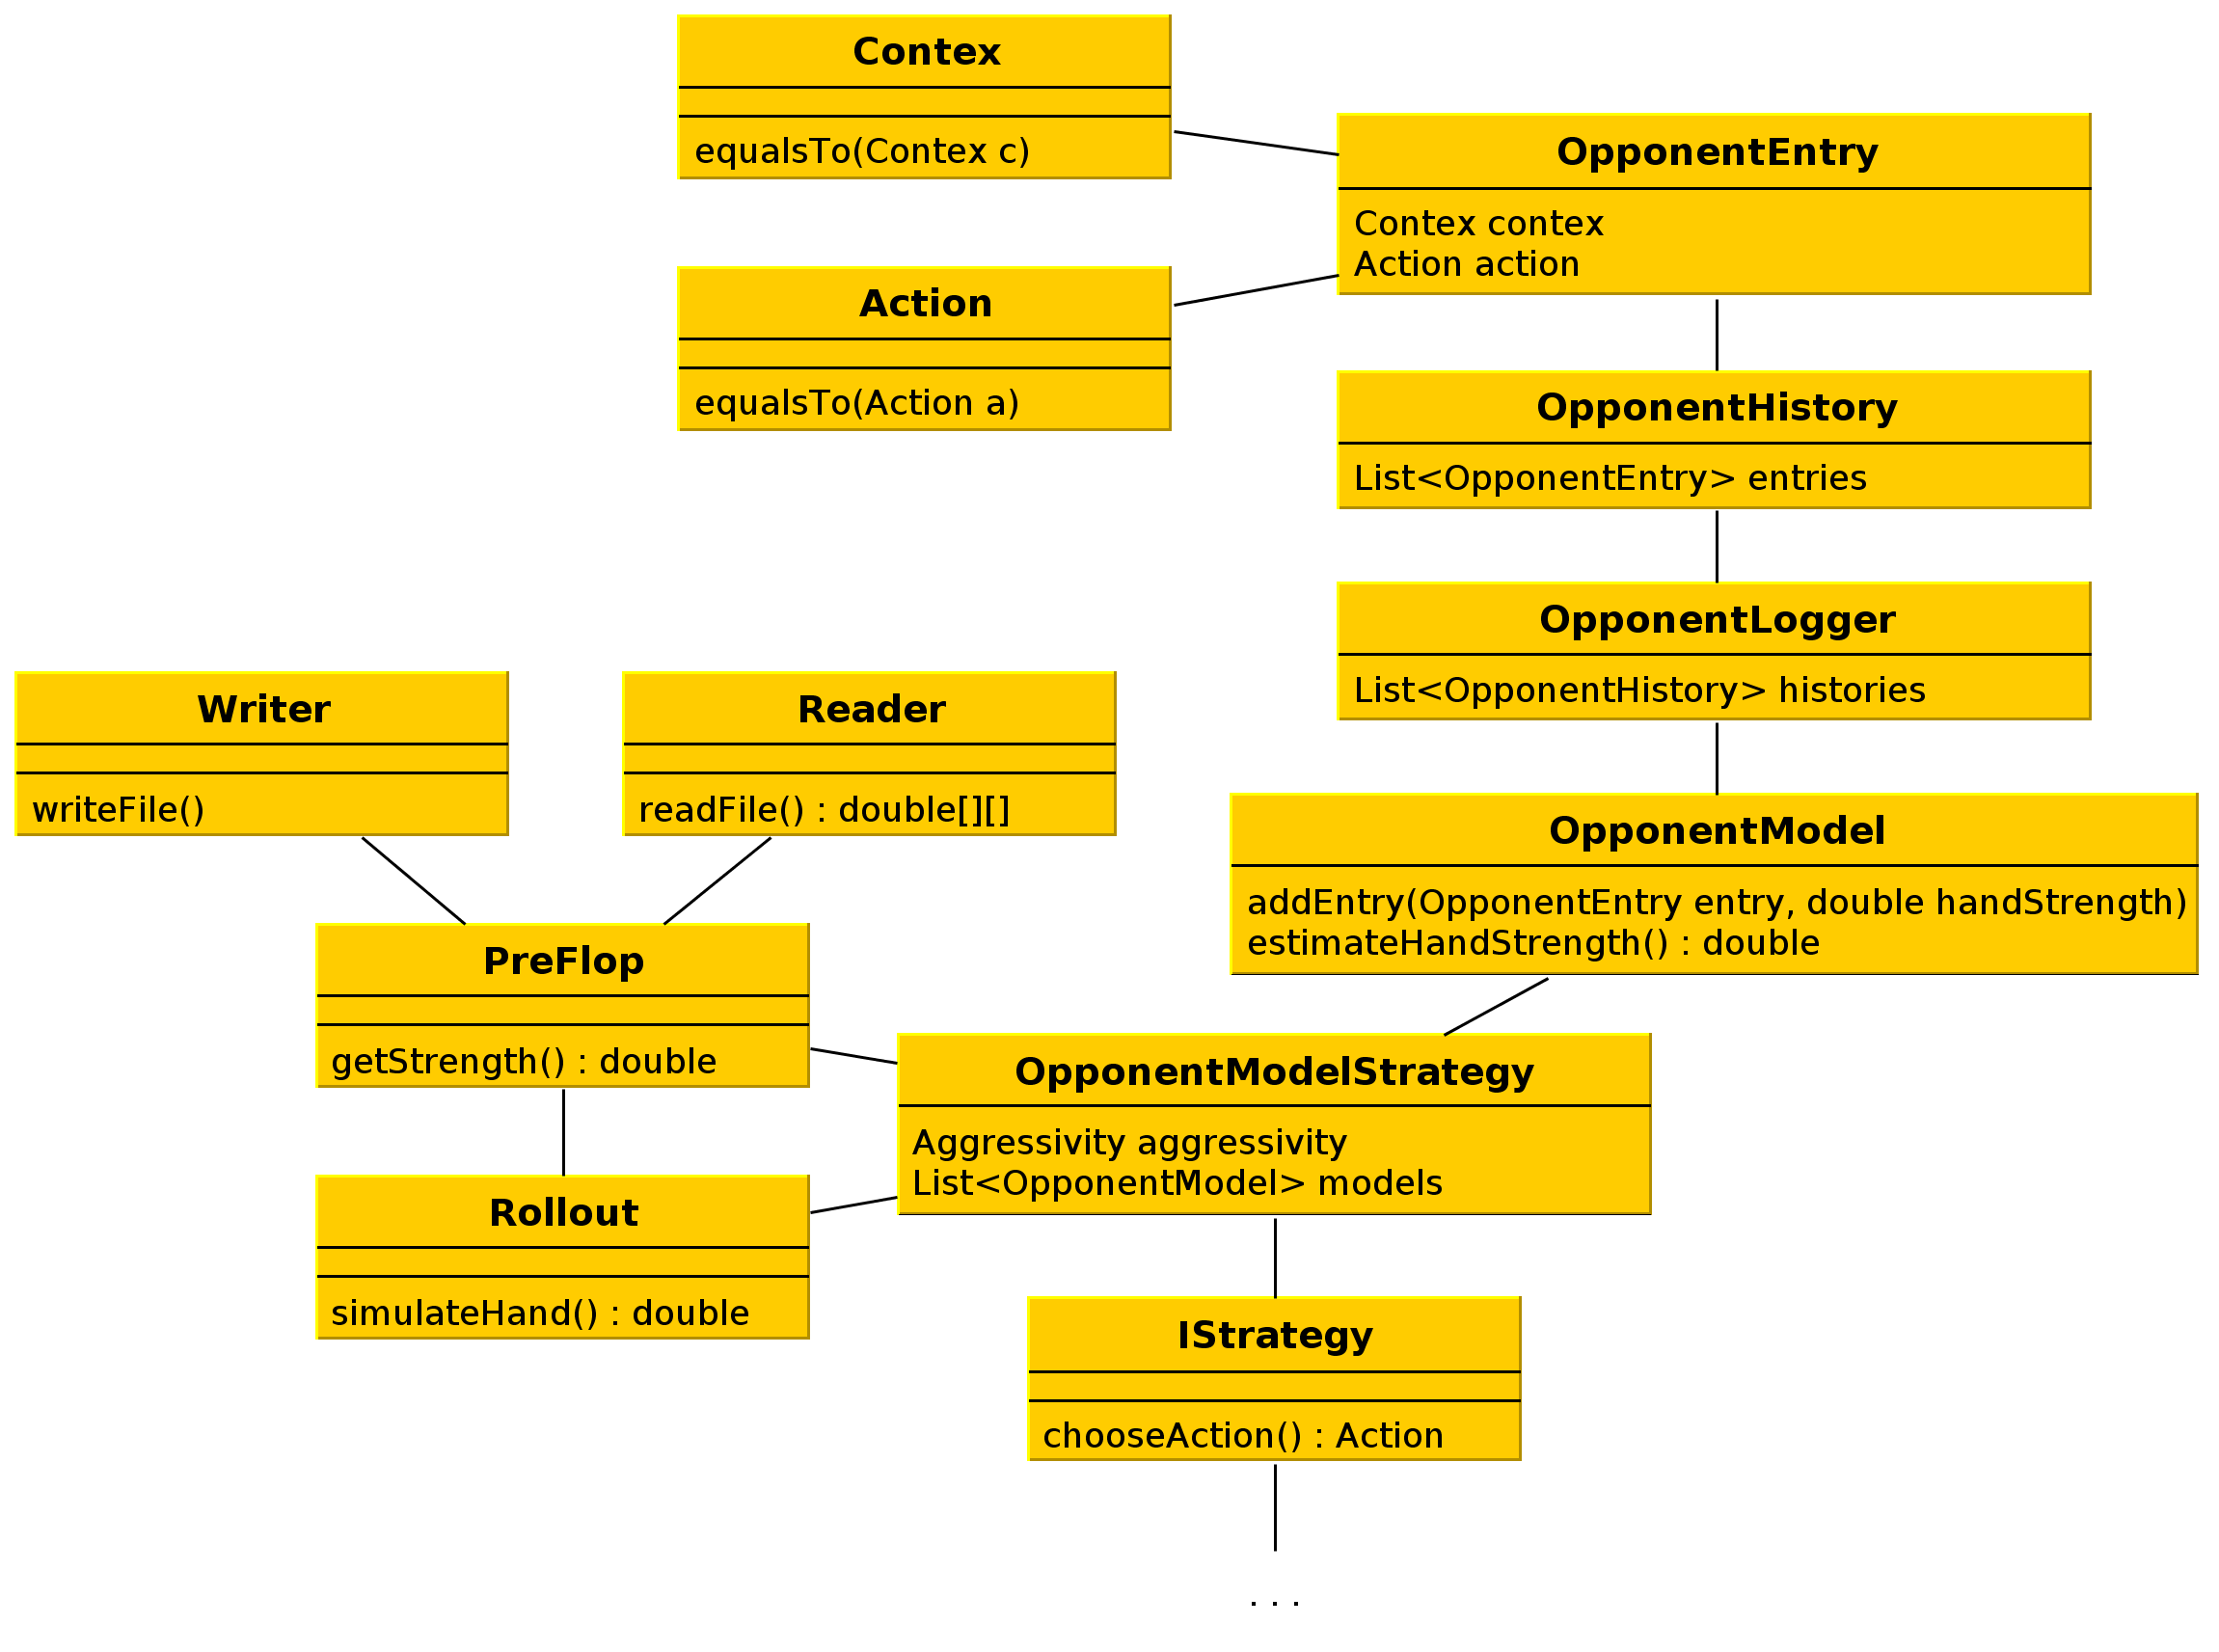
\includegraphics[width=1.0\textwidth]{images/phase3}
  \caption{Software design of phase III}
  \label{fig:phase3}
\end{figure}

\section{Model rules}
As mentioned above, the \emph{Opponent Model} contains  a triple of \emph{Context}, \emph{Player Action} and \emph{Hand Strength} of which the first two are again subdevided.

\subsection{Context}
The \emph{Context} can be considered as the state of the game at a specific point. Features that define a context are 
\begin{itemize}
	\item The stage, whether pre-flop, flop, turn or river
	\item The number of player that are still in the hand
	\item The number of raises during the current stage
	\item The pott odds
\end{itemize}

However, in order to estimate a player's hand in a given context correctly, the context have to be neither too general nor too specific. Therefore, the mentioned features have to be grouped into classes. For example, the pot odds of 0.20 and 0.21 should be considered the same. The classes that are used for the \emph{Opponent model strategy} are 
\begin{itemize}
	\item \textbf{The stage:} pre-flop, flop, turn or river
	\item \textbf{The number of player:} 1 to 3, 4 to 7 and 8 to 10
	\item \textbf{The number of raises:} 1 to 2 and more than 3
	\item \textbf{The pott odds:} 0.0 to 0.3 and more than 0.3
\end{itemize}

\subsection{Player Action}
The information about a player's action is also subdevided in classes.
\begin{itemize}
	\item \textbf{The action:}  call or raise
	\item \textbf{The bet:} 1 to 500 and more than 500
\end{itemize}
There are no fold entries in the \emph{Opponent Model} because folded cards never reach the showdown and therefore are never shown. 

\section{Opponent Model Strategy}
Basically the phase III player acts the same way like phase II player does. At first the amount that a player is willing to pay is calculated the same way. Afterwards the opponents' hand strengths are estimated. The player compares his own hand strengths with the estimated strengths and gets a number of players who are supposedly better and worse than him. These numbers are used to adjust the player's bet. The new bet is calculated as shown in \ref{equ:opponentModel1}, where $b'$ is the new bet, $b$ the old bet, $better$ the number of players who are better and $worse$ the number of player who are worse than the current player.
\begin{equation}
	\label{equ:opponentModel1}
	b' = b * (\frac{worse - better}{10})
\end{equation}

At the beginning, when there are very few hands played and the model has almost no entries, the estimated number of better/worse players will be close to zero. That means that there is no adjustment to the bet and the player plays exactly the way the phase II player does. As the number of played hands rises, the model will have more information about the players and the bet will be adjusted more often.

\section{Results}

